% Part 5: the interpretation of the two halves of the cosmological virial partition.
% Carried line by line from: Dark Matter and Dark Energy as Virial Partners: The Geometric and Kinetic Halves of a Single Cosmological Virial Equilibrium
% (Mar 2026; abstract, sections 1, 2 (interpretation), 3, 3.1, 3.2, 5, 6, 8, Fig. 2); The Virial Partition Across Wide Range of Physical Scales
% (25 Feb 2026; section 3.3, the three-channel decomposition, and the interpretive paragraph of section 8).
% The observational sections of the same papers are in Part 2 (Chapters ch:virial, ch:virial_tests).
% Corrections applied: errata V1, V4, V5, V12 (carried as conjecture, the author's ruling pending), V22; VIRIAL_CHECK.md items 3-5, 12; ledger note 11(g).
% Numbers: docs/verification/scripts/verify_virial_papers.py (section G); figure: docs/book/figscripts/fig_virial_book.py (fig_virial_partition).

\chapter{Dark matter and dark energy as virial partners}\label{ch:virial_partners}

\section*{Overview}
The coupling constant $\beta_m=\Omega_m/2$ is derived from the virial theorem applied to gravitational decoherence (Chapter~\ref{ch:virial}). This
derivation carries a direct physical interpretation: the $1/2$ partition divides gravitational energy between its geometric potential half, stored in
spacetime curvature, and its kinetic informational half, accumulated as Landauer pressure on the cosmological horizon. What observational cosmology
identifies as dark matter is the potential half. What it identifies as dark energy is the kinetic half, together with the vacuum baseline. These are not two
phenomena requiring separate explanations. They are two expressions of the equilibrium condition $2K+V=0$ operating at cosmological scales.
\conjecture\ The virial ratio $\Omega_ma^{-3}/[\beta_mE(a)]$ descends from effectively infinite at early times to exactly $2.0$ at $a=1$ --- not as a
fine-tuning, but, on this reading, as the universe reaching its epoch of first cosmological virialisation. The coincidence problem is not a problem; it is a
consequence. \interp\ This chapter presents the identification, the consistency of the data with it (set out in full in Chapters~\ref{ch:virial}
and~\ref{ch:virial_tests}), the limits of current data, and the question the framework forces: if the kinetic half crosses into classical actuality at each
decoherence event, and the potential half encodes into surrounding spacetime geometry, what is spacetime geometry made of?

\section{The problem with two mysteries}\label{sec:vp_problem}
The standard cosmological model accounts for 95\,\% of the energy content of the universe with two entries whose physical nature remains unknown. Dark
matter, inferred from the discrepancy between observed gravitational effects and visible mass, constitutes approximately 26\,\% of the critical density.
Dark energy, inferred from the observed acceleration of cosmic expansion, constitutes approximately 69\,\%. These two components are treated as independent
phenomena, described by separate theoretical frameworks, and pursued by separate experimental programmes.

This separation has always had an uncomfortable feature. The ratio of dark matter to dark energy density today --- approximately 0.38 --- is coincidentally
close to $1/2$ only for observers living near the present epoch. \calc\ At earlier times, matter density scales as $a^{-3}$ while the cosmological constant
remains fixed, so their ratio was enormous in the past and will be negligible in the future. The fact that we observe them as comparable today has no
explanation within the standard model beyond anthropic selection. This is the coincidence problem.

A separate but related observation: the coupling constant that governs IAM's late-time growth suppression, $\beta_m=\Omega_m/2$, is derived from the virial
theorem. The virial theorem~\cite{Clausius1870} states that for any system bound by a $1/r$ potential --- gravitational or Coulomb --- the time-averaged kinetic and potential
energies satisfy $2\langle K\rangle+\langle V\rangle=0$. This has been verified from atomic scales ($10^{-11}$\,m) to clusters of galaxies, at machine
precision for quantum mechanical systems, and it fixes the coupling at the cosmic horizon ($10^{26}$\,m), where the Planck chains are consistent with it
(Chapter~\ref{ch:virial_law}).

The question that arises naturally from these two observations is: why does the virial theorem, an equilibrium condition for bound gravitational systems,
produce the coupling constant for a cosmological energy density? And why is the ratio of matter to the record term today the virial ratio of 2? The
answer proposed here is the same in both cases.

\section{The cosmological virial partition}\label{sec:vp_partition}
The physical interpretation of Eq.~\eqref{eq:vc_beta} is the central argument of this chapter. \conjecture

The virial theorem partitions gravitational energy into two equal halves. In IAM, one half deposits into spacetime geometry as curvature --- the potential
half, stored in the gravitational configuration of collapsed structures. The other half crosses into classical actuality as kinetic informational energy
--- the kinetic half, accumulated as Landauer pressure on the cosmological horizon and driving the late-time modification to matter perturbation growth.

What observational cosmology identifies as dark matter is the potential half. The gravitational effects attributed to dark matter --- excess curvature in
galaxies and clusters beyond what baryonic matter alone would produce --- are the geometric reservoir of deposited potential energy. This is not a particle.
It is the geometric consequence of the virial partition operating continuously across cosmic history. The identification has to face every phenomenological
success of particle dark matter at once --- the CMB peak heights, the lensing offset of merging clusters, structure formation before recombination
(Chapter~\ref{ch:time}).

What observational cosmology identifies as dark energy is the kinetic half. The accumulated Landauer costs of gravitational decoherence events, encoded on
the horizon, produce an informational pressure that modifies the late-time expansion environment for matter. The cosmological constant $\Lambda$ is the
vacuum baseline --- the minimum Landauer payment required to maintain the virial equilibrium of empty spacetime (Chapter~\ref{ch:lambda}). The dynamically
growing component, $\beta_mE(a)$, is the kinetic half accumulating as structure forms.

These are not two separate phenomena. They are the two sides of the same balance sheet, required to be equal by the theorem that governs every $1/r$
potential in nature.

\section{The virial ratio through cosmic history}\label{sec:vp_ratio}
The cosmological virial ratio $R(a)=\Omega_ma^{-3}/[\beta_mE(a)]$ (Eq.~\eqref{eq:vc_R}) measures the potential half against the kinetic half. At early
times, $E(a)\approx0$ and the kinetic half has not yet activated --- the universe is almost entirely potential, unactivated geometric storage. The ratio
$R(a)$ is effectively infinite. As structure forms and decoherence events accumulate, the kinetic half grows: $R=399$ at $z=2$, $20$ at $z=0.7$, $6$ at
$z=0.3$ (Table~\ref{tab:vc_R}). \calc\ At $a=1$, by construction, $R(1)=\Omega_m/[\beta_mE(1)]=2$.

The value 2 today is the definition $\beta_m=\Omega_m/2$ together with $E(1)=1$; the reading is what gives it content. The ratio $|V|/K=2$ is the
equilibrium condition, and on this reading the universe has been approaching it throughout its history. Today is the epoch when cosmological
virialisation is first achieved. The kinetic half has finally activated enough --- $E(a)$ has grown from zero to one --- to bring the ratio to 2. \interp

\section{The coincidence problem dissolved}\label{sec:vp_coincidence}
The standard coincidence problem asks why $\Omega_m$ and $\Omega_\Lambda$ are comparable today. Under the virial partition interpretation, this is not a
coincidence requiring an explanation. It is the equilibrium condition. The kinetic half and the potential half must be in the ratio $1:2$ for the system to
be virialised. The universe has been spending its entire history paying down that ratio. The epoch at which $R(a)=2$ is not special because we happen to
live in it. It is special because $E(a{=}1)=1$ by derivation from the Gibbons--Hawking temperature of the de Sitter horizon, and $a=1$ is now by
definition. Any sufficiently complex observer must exist after enough structure has formed to support them --- which is precisely the epoch when $E(a)$ is
approaching unity. The anthropic selection and the physics point to the same moment. \interp

\section{The virial ratio as a figure of merit}\label{sec:vp_merit}

\begin{figure}[htbp]\centering
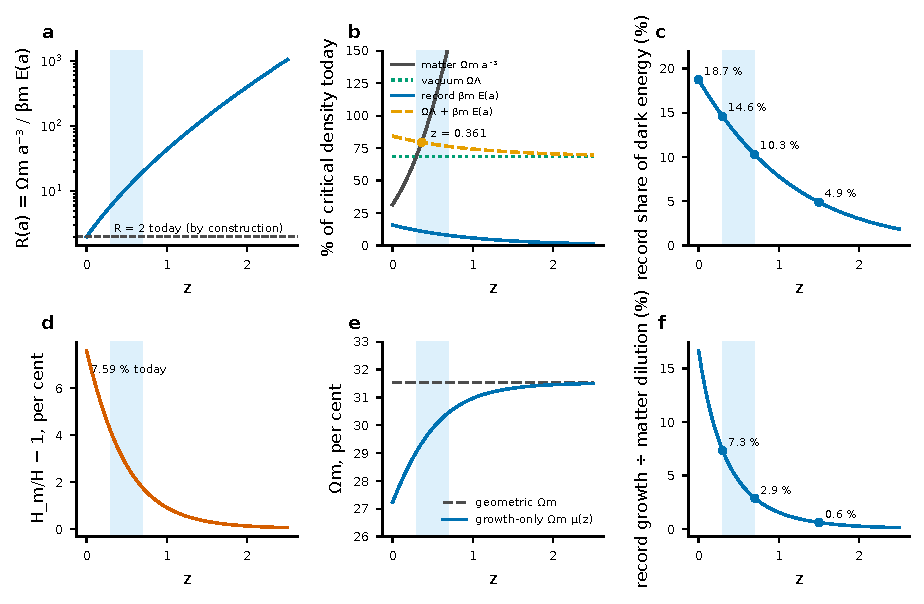
\includegraphics[width=\textwidth]{figures/part5/fig_virial_partition.pdf}
\caption{The cosmological virial partition through the transition zone ($z\approx0.3$--$0.7$, shaded in all panels). (a) The virial ratio $R(a)=\Omega_ma^{-3}/[\beta_mE(a)]$ descends from large values at early times to exactly 2 at $z=0$, by construction. (b) Energy budget: the potential half ($\Omega_ma^{-3}$), the vacuum floor ($\Omega_\Lambda$), the kinetic informational half ($\beta_mE(a)$) and their dark-energy sum; matter equals the sum at $z=0.361$ ($\Lambda$CDM: 0.295). (c) The record term as a fraction of the total dark energy, $\beta_mE/(\Omega_\Lambda+\beta_mE)$: 4.9\,\% at $z=1.5$ growing to 18.7\,\% today. (d) The gap between the matter-sector and photon-sector expansion rates, $H_m/H-1=\mu^{-1/2}-1$: 7.59\,\% today. (e) The growth-only $\Omega_m\mu(z)$ against the geometric $\Omega_m$. (f) The rate of growth of the kinetic half relative to the rate of matter dilution, $[d(\beta_mE)/da]/|d(\Omega_ma^{-3})/da|=E(a)a^2/6$: 7.3, 2.9 and 0.6\,\% at $z=0.3$, 0.7 and 1.5. Planck 2018 background, $\beta_m=0.15765$; all curves follow from $\beta_m=\Omega_m/2$ with no fitted parameters. \calc}\label{fig:virial_partition}
\end{figure}
Figure~\ref{fig:virial_partition} shows the cosmological virial ratio $R(a)$, the energy budget of the dark sector, the informational pressure growth
rate, the sector gap, and the growth--geometry discrepancy. The transition zone ($z\approx0.3$--$0.7$) is the observational window in which the kinetic half
is most actively growing relative to the potential half and where the predictions are most distinguishable from $\Lambda$CDM. In it the informational
pressure is 10--15\,\% of the total dark energy, the virial ratio runs from 6 to 20, and the growth-only $\Omega_m$ lies 3--8\,\% below the geometric value.
\calc\ Today the record term is 18.7\,\% of the dark energy, $\beta_m/(\Omega_\Lambda+\beta_m)$. \calc

\section{The three channels of $\beta_m$}\label{sec:vp_channels}
An informational virial analysis decomposes $\beta_m$ into three physically distinct channels:
{\small\begin{align}
\beta_{\rm temporal}&=0.076618\ (48.6\,\%):&&\text{kinetic decoherence events}\to\sigma_8,\ f\sigma_8,\ \text{RSD},\nonumber\\
\beta_{\rm geometric}&=0.078825\ (50.0\,\%):&&\text{structural configuration bits}\to\text{lensing/dynamics ratio},\label{eq:vp_channels}\\
\beta_{\rm radiative}&=0.002207\ (1.4\,\%):&&\text{photon-transmitted information}\to\text{SZ/X-ray/lensing cluster ratio}.\nonumber
\end{align}}
The sum $\beta_{\rm total}=0.15765=\Omega_m/2$, and $\beta_{\rm geometric}=\beta_m/2$ exactly. \calc\ The radiative channel is not a rounding residual: it is
read as the fraction of gravitational binding energy transmitted as photon radiation, and it would set the three-way cluster test of
Section~\ref{sec:vt_cluster}. The decomposition is derived from the same virial partition as $\beta_m$ itself; the split of the temporal half into the temporal and radiative channels is taken as given here, and its derivation, with independent cluster measurement, is the next step. \conjecture\ \openprob

\section{A question the framework forces}\label{sec:vp_question}
The identification developed in the preceding sections has an implication that is stated as a question rather than a claim, because it reaches beyond what
can currently be tested. \conjecture

In the IAM mechanism, each gravitational decoherence event partitions gravitational energy. The kinetic half crosses into classical actuality as observable
energy --- baryonic dynamics, radiation, the thermodynamic irreversibility that constitutes the arrow of time. The Landauer cost of that crossing encodes
on the cosmological horizon. This is the half we call dark energy.

The potential half deposits into the surrounding spacetime geometry as curvature. This is the half we call dark matter. It does not oscillate. It is not a
particle. It is the geometric record of every virialisation event that has ever occurred, stored in the curvature of spacetime itself. In the ratio $R(a)$
this half enters as the matter density $\Omega_ma^{-3}$, which dilutes with expansion; what accumulates, on this reading, is the record itself, the
integral of deposits, not its density. How the two statements fit together is part of the question. \openprob

If this identification is correct, then the geometry of spacetime is not a pre-existing medium on which information is written. It is the accumulated
integral of every potential-half deposit from every decoherence event in cosmic history. Expansion is not making room for information encoding. Expansion is
the accumulation of deposits. The geometry is not deformed by matter. The geometry is constituted by matter's continuous transition from potential to actual.

This raises an open question:
\begin{quote}
If the potential half of each decoherence event encodes into spacetime geometry, what is spacetime geometry made of?
\end{quote}
It is the question that follows from taking the virial partition seriously at the cosmological level, and the
observational programme now underway will determine whether it is the right question to ask.

\section{Conclusions}\label{sec:vp_conclusions}
The $1/2$ partition in IAM's coupling constant $\beta_m=\Omega_m/2$ is not, on this reading, a calculational step. It is a physical identification. The
virial theorem divides gravitational energy between two halves, and those two halves are what cosmology has been calling dark matter and dark energy.
\conjecture

The potential half is stored in spacetime curvature. It records the geometric consequences of every virialisation event in cosmic history. It is what we
infer as dark matter from the discrepancy between observed gravitational effects and visible mass.

The kinetic half crosses into classical actuality at each decoherence event, accumulating on the cosmological horizon as Landauer pressure. It drives the
late-time modification to structure growth that IAM predicts and that the current data are consistent with. It is, together with the vacuum baseline
$\Lambda$, what we infer as dark energy from the observed acceleration of expansion.

The coincidence problem --- why these two densities are comparable today --- is not a problem under this identification. It is the statement that the
universe has reached its epoch of first cosmological virialisation. The ratio $R(a)=\Omega_ma^{-3}/[\beta_mE(a)]$ arrives at exactly $2.0$ at $a=1$ because
$\beta_m=\Omega_m/2$ by the virial theorem and $E(1)=1$ by the thermodynamic derivation from the de Sitter horizon. These two facts together mean the
universe has been continuously approaching the virial equilibrium since the beginning, and arrives there now. \interp

The question the framework forces --- what spacetime geometry is made of if it is the deposited potential half of every decoherence event in cosmic
history --- is left open. It is the question that follows from taking the result seriously, and it is not answered by the data that exist today.

What is answered by the data is whether the sector split is real. Euclid and DESI Year~5 will measure it (Chapter~\ref{ch:virial_tests}). The prediction is
on record: $\mu_0=-0.136$, $\Sigma_0=0$. \prediction

The interpretive paragraph of the cross-domain analysis states the same view at every scale: the virial $1/2$ partition divides gravitational energy
between geometric entropy (spacetime curvature) and informational entropy (gravitational decoherence), and the division propagates from the quantum scale
(Landauer's principle, $k_BT\ln2$ per bit) to the cosmic scale ($\mu_0=-0.136$ suppressing matter growth while leaving photons unmodified). \interp

This is a clean target: a fixed coupling, dated surveys, and a question about what spacetime geometry is made of. A cosmologist can run the growth and lensing chains now; a relativist can take up the question itself.
